\documentclass[preview,border=7mm]{standalone}
\usepackage[T1]{fontenc}
\usepackage{lmodern}
\usepackage{xcolor}
\usepackage{xinttools}
\usepackage{tikz}
\usetikzlibrary{calc,positioning,arrows.meta,shadows,backgrounds,fit,shapes.geometric}

% Inspired by:
% 1) SWAN wave model - TeXample.net: slanted computational/grid layer idea
%    https://texample.net/swan-wave-model/
% 2) Database decimation process - TeXample.net: repeated computed blocks and TikZ-side sizing math
%    https://texample.net/database-decimation-process/
% 3) Network Topology - TeXample.net: topology-style boxes, shadows, and stacked infrastructure look
%    https://texample.net/network-topology/

\begin{document}
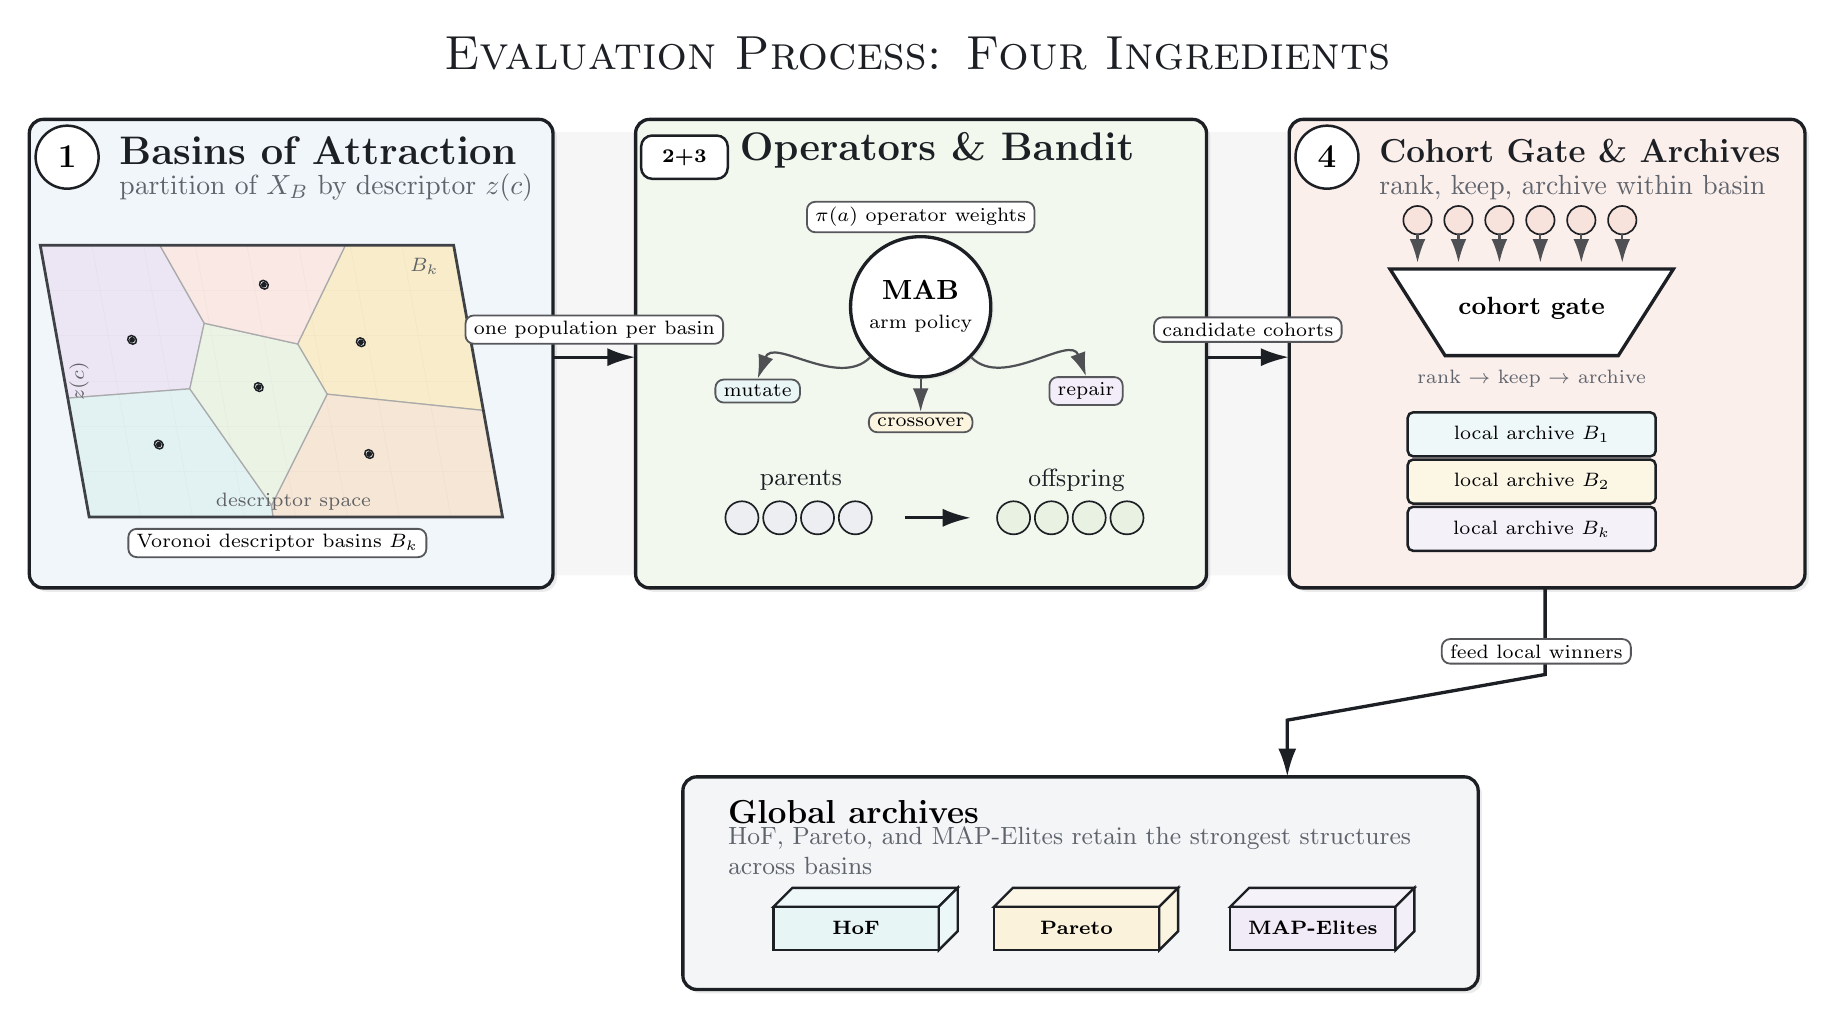
\begin{tikzpicture}[x=1cm,y=1cm]

% =========================================================
% Computed geometry: all main coordinates derive from these.
% =========================================================
\pgfmathsetmacro{\PanelH}{5.95}
\pgfmathsetmacro{\PoneW}{6.65}
\pgfmathsetmacro{\PtwoW}{7.25}
\pgfmathsetmacro{\PfourW}{6.55}
\pgfmathsetmacro{\Gap}{1.05}
\pgfmathsetmacro{\Xone}{0.0}
\pgfmathsetmacro{\Xtwo}{\Xone+\PoneW+\Gap}
\pgfmathsetmacro{\Xfour}{\Xtwo+\PtwoW+\Gap}
\pgfmathsetmacro{\Ytop}{0.0}
\pgfmathsetmacro{\ArchiveW}{10.10}
\pgfmathsetmacro{\ArchiveH}{2.70}
\pgfmathsetmacro{\ArchiveX}{\Xtwo+0.60}
\pgfmathsetmacro{\ArchiveY}{-8.35}
\pgfmathsetmacro{\TotalW}{\PoneW+\PtwoW+\PfourW+2*\Gap}
\pgfmathsetmacro{\TitleX}{\TotalW/2}

% =========================================================
% Colors
% =========================================================
\definecolor{ink}{RGB}{28,31,36}
\definecolor{muted}{RGB}{94,99,108}
\definecolor{paper}{RGB}{250,249,246}
\definecolor{blueA}{RGB}{218,232,244}
\definecolor{greenA}{RGB}{224,237,214}
\definecolor{redA}{RGB}{244,208,198}
\definecolor{goldA}{RGB}{246,230,181}
\definecolor{violetA}{RGB}{226,216,239}
\definecolor{cyanA}{RGB}{209,235,236}
\definecolor{orangeA}{RGB}{244,221,197}
\definecolor{grayA}{RGB}{232,234,238}

% =========================================================
% Styles
% =========================================================
\tikzset{
  panel/.style={
    draw=ink,
    very thick,
    rounded corners=5pt,
    fill=paper,
    drop shadow={opacity=.16,shadow xshift=1.4pt,shadow yshift=-1.4pt}
  },
  tag/.style={
    circle,
    draw=ink,
    line width=.9pt,
    fill=white,
    minimum size=8mm,
    inner sep=0pt,
    font=\bfseries\large
  },
  tagwide/.style={
    rounded corners=4pt,
    draw=ink,
    line width=.9pt,
    fill=white,
    minimum width=14mm,
    minimum height=8mm,
    inner sep=1pt,
    font=\bfseries\normalsize
  },
  title/.style={font=\bfseries\fontsize{13.4}{15.2}\selectfont, text=ink, anchor=west},
  subtitle/.style={font=\fontsize{10.2}{12}\selectfont, text=muted, anchor=west, align=left},
  tinylabel/.style={font=\scriptsize, text=ink, align=center},
  smalllabel/.style={font=\small, text=ink, align=center},
  flow/.style={-{Latex[length=3.6mm,width=2.3mm]}, very thick, draw=ink},
  softflow/.style={-{Latex[length=3.0mm,width=2.0mm]}, thick, draw=ink!78},
  dot/.style={circle, fill=ink, inner sep=0pt, minimum size=2.1pt},
  candidate/.style={circle, draw=ink, line width=.6pt, fill=white, minimum size=4.2mm, inner sep=0pt},
  chip/.style={rounded corners=3pt, draw=ink!75, fill=white, line width=.65pt, font=\scriptsize, inner xsep=3pt, inner ysep=2pt},
  drawer/.style={draw=ink, line width=.9pt, rounded corners=2pt, fill=white, minimum width=3.15cm, minimum height=.56cm, font=\scriptsize}
}

% =========================================================
% Title
% =========================================================
\node[font=\scshape\fontsize{18}{20}\selectfont, text=ink] at (\TitleX,0.84) {Evaluation Process: Four Ingredients};

% =========================================================
% Panel backgrounds
% =========================================================
\path[panel, fill=blueA!38]  (\Xone,\Ytop) rectangle ++(\PoneW,-\PanelH);
\path[panel, fill=greenA!38] (\Xtwo,\Ytop) rectangle ++(\PtwoW,-\PanelH);
\path[panel, fill=redA!35]   (\Xfour,\Ytop) rectangle ++(\PfourW,-\PanelH);

% step tags
\node[tag] at ($(\Xone,\Ytop)+(.48,-.48)$) {1};
\node[
  tagwide,
  minimum width=11mm,
  minimum height=5.5mm,
  inner xsep=1pt,
  inner ysep=0.5pt,
  font=\scriptsize\bfseries
] at ($(\Xtwo,\Ytop)+(.62,-.48)$) {2+3};
\node[tag] at ($(\Xfour,\Ytop)+(.48,-.48)$) {4};

% headings
\node[title] at ($(\Xone,\Ytop)+(1.02,-.40)$) {Basins of Attraction};
\node[subtitle] at ($(\Xone,\Ytop)+(1.02,-.86)$) {partition of $X_B$ by descriptor $z(c)$};

\node[title] at ($(\Xtwo,\Ytop)+(1.20,-.40)$) {Operators \& Bandit};
\node[title, font=\bfseries\fontsize{12.4}{14.0}\selectfont] at ($(\Xfour,\Ytop)+(1.02,-.40)$) {Cohort Gate \& Archives};
\node[subtitle] at ($(\Xfour,\Ytop)+(1.02,-.86)$) {rank, keep, archive within basin};

% =========================================================
% Stage 1: slanted Voronoi basin map, adapted from the Voronoi clipping idea
% while preserving the original SWAN-like slanted grid panel.
% The Voronoi polygons are precomputed from fixed sites inside the descriptor rectangle,
% so the figure compiles reliably with pdflatex.
% =========================================================
\begin{scope}[shift={(\Xone+0.76,\Ytop-5.05)},xslant=-0.18]
  \fill[white, opacity=.88] (0,0) rectangle (5.25,3.45);

  % soft computational grid kept from the previous pretty version
  \foreach \i in {1,...,7}{
    \pgfmathsetmacro{\xx}{\i*5.25/8}
    \draw[ink!16, line width=.35pt] (\xx,0) -- (\xx,3.45);
  }
  \foreach \j in {1,...,5}{
    \pgfmathsetmacro{\yy}{\j*3.45/6}
    \draw[ink!16, line width=.35pt] (0,\yy) -- (5.25,\yy);
  }

  % Voronoi cells in descriptor space
  \filldraw[fill=violetA!74, draw=ink!40, line width=.45pt, opacity=.86]
    (0.000,1.510) -- (1.571,1.628) -- (1.904,2.461) -- (1.519,3.450) -- (0.000,3.450) -- cycle;
  \filldraw[fill=goldA!82, draw=ink!40, line width=.45pt, opacity=.86]
    (3.043,2.198) -- (3.303,1.560) -- (5.250,1.354) -- (5.250,3.450) -- (3.874,3.450) -- cycle;
  \filldraw[fill=cyanA!72, draw=ink!40, line width=.45pt, opacity=.86]
    (2.343,0.148) -- (1.571,1.628) -- (0.000,1.510) -- (0.000,0.000) -- (2.336,0.000) -- cycle;
  \filldraw[fill=orangeA!82, draw=ink!40, line width=.45pt, opacity=.86]
    (3.303,1.560) -- (2.343,0.148) -- (2.336,0.000) -- (5.250,0.000) -- (5.250,1.354) -- cycle;
  \filldraw[fill=greenA!70, draw=ink!40, line width=.45pt, opacity=.86]
    (1.904,2.461) -- (1.571,1.628) -- (2.343,0.148) -- (3.303,1.560) -- (3.043,2.198) -- cycle;
  \filldraw[fill=redA!55, draw=ink!40, line width=.45pt, opacity=.86]
    (1.904,2.461) -- (3.043,2.198) -- (3.874,3.450) -- (1.519,3.450) -- cycle;

  % Voronoi sites / basin representatives
  \foreach \bx/\by in {0.95/2.25,3.85/2.22,1.05/0.92,3.70/0.80,2.45/1.65,2.75/2.95}{
    \filldraw[fill=white, draw=ink, line width=.55pt] (\bx,\by) circle (.055);
    \node[dot] at (\bx,\by) {};
  }

  \node[font=\scriptsize, text=ink!70] at (2.63,.20) {descriptor space};
  \node[font=\scriptsize, text=ink!70, rotate=90] at (.18,1.72) {$z(c)$};
  \node[font=\scriptsize, text=ink!70] at (4.83,3.18) {$B_k$};

  \draw[ink!85, line width=1.0pt] (0,0) rectangle (5.25,3.45);
\end{scope}
\node[chip] at ($(\Xone,\Ytop)+(3.15,-5.38)$) {Voronoi descriptor basins $B_k$};
% =========================================================
% Stage 2+3: operator policy and candidate production
% =========================================================
\coordinate (hub) at ($(\Xtwo,\Ytop)+(3.62,-2.38)$);
\node[circle, draw=ink, very thick, fill=white, minimum size=1.28cm, align=center,
      drop shadow={opacity=.10,shadow xshift=1pt,shadow yshift=-1pt}] (bandit) at (hub)
      {\bfseries MAB\\[-.15em]\scriptsize arm policy};

\node[chip, fill=cyanA!45]   (muta) at ($(\Xtwo,\Ytop)+(1.55,-3.45)$) {mutate};
\node[chip, fill=goldA!45]   (cross) at ($(\Xtwo,\Ytop)+(3.62,-3.85)$) {crossover};
\node[chip, fill=violetA!45] (rep) at ($(\Xtwo,\Ytop)+(5.72,-3.45)$) {repair};

\draw[softflow] (bandit.south west) to[out=225,in=70] (muta.north);
\draw[softflow] (bandit.south)      -- (cross.north);
\draw[softflow] (bandit.south east) to[out=315,in=110] (rep.north);

% Parent and offspring rows, computed repeated candidate circles.
\node[smalllabel] at ($(\Xtwo,\Ytop)+(2.1,-4.58)$) {parents};
\foreach \i in {0,...,3}{
  \pgfmathsetmacro{\px}{\Xtwo+1.85+\i*.48}
  \node[candidate, fill=grayA!80] (p\i) at (\px - 0.5 ,\Ytop-5.06) {};
}

\draw[flow] ($(\Xtwo,\Ytop)+(3.42,-5.06)$) -- ($(\Xtwo,\Ytop)+(4.26,-5.06)$);
\node[smalllabel] at ($(\Xtwo,\Ytop)+(5.6,-4.58)$) {offspring};
\foreach \i in {0,...,3}{
  \pgfmathsetmacro{\ox}{\Xtwo+5.30+\i*.48}
  \node[candidate, fill=greenA!70] (o\i) at (\ox - 0.5,\Ytop-5.06) {};
}

\node[chip, fill=white] at ($(\Xtwo,\Ytop)+(3.62,-1.24)$) {$\pi(a)$ operator weights};

% =========================================================
% Stage 4: cohort gate, local archive drawers
% =========================================================
\begin{scope}[shift={(\Xfour+1.08,\Ytop-2.45)}]
  % funnel/gate
  \path[draw=ink, very thick, fill=white]
    (0.20,0.55) -- (3.80,0.55) -- (3.10,-0.55) -- (0.90,-0.55) -- cycle;
  \node[font=\bfseries\small] at (2.00,.05) {cohort gate};
  \node[font=\scriptsize, text=muted] at (2.00,-.84) {rank $\rightarrow$ keep $\rightarrow$ archive};

  % incoming cohort dots
  \foreach \i in {0,...,5}{
    \pgfmathsetmacro{\cx}{.55+\i*.52}
    \node[candidate, fill=redA!62, minimum size=3.6mm] at (\cx,1.17) {};
    \draw[softflow] (\cx,1.00) -- (\cx,.63);
  }

  % archive drawers
  \node[drawer, fill=cyanA!35]   at (2.00,-1.55) {local archive $B_1$};
  \node[drawer, fill=goldA!35]   at (2.00,-2.15) {local archive $B_2$};
  \node[drawer, fill=violetA!35] at (2.00,-2.75) {local archive $B_k$};
\end{scope}

% =========================================================
% Global archives: topology/stacked infrastructure style
% =========================================================
\path[panel, fill=grayA!48] (\ArchiveX,\ArchiveY) rectangle ++(\ArchiveW,-\ArchiveH);
\node[font=\bfseries\large, anchor=west] at ($(\ArchiveX,\ArchiveY)+(.45,-.44)$) {Global archives};
\node[font=\small, text=muted, anchor=west, align=left, text width=8.95cm] at ($(\ArchiveX,\ArchiveY)+(.45,-.94)$) {HoF, Pareto, and MAP-Elites retain the strongest structures across basins};

% Macro-like repeated 3D blocks drawn manually, no custom shape required.
\newcommand{\archiveblock}[4]{%
  \begin{scope}[shift={(#1,#2)}]
    \path[draw=ink, line width=.85pt, fill=#4!50] (0,0) rectangle (2.10,.55);
    \path[draw=ink, line width=.85pt, fill=#4!34] (0,.55) -- (.24,.79) -- (2.34,.79) -- (2.10,.55) -- cycle;
    \path[draw=ink, line width=.85pt, fill=#4!42] (2.10,0) -- (2.34,.24) -- (2.34,.79) -- (2.10,.55) -- cycle;
    \node[font=\bfseries\scriptsize] at (1.05,.28) {#3};
  \end{scope}
}
\archiveblock{\ArchiveX+1.15}{\ArchiveY-2.20}{HoF}{cyanA}
\archiveblock{\ArchiveX+3.95}{\ArchiveY-2.20}{Pareto}{goldA}
\archiveblock{\ArchiveX+6.95}{\ArchiveY-2.20}{MAP-Elites}{violetA}

% =========================================================
% Inter-panel arrows with midpoint labels.
% =========================================================
\coordinate (p1out) at (\Xone+\PoneW,\Ytop-3.02);
\coordinate (p2in)  at (\Xtwo,\Ytop-3.02);
\coordinate (p2out) at (\Xtwo+\PtwoW,\Ytop-3.02);
\coordinate (p4in)  at (\Xfour,\Ytop-3.02);
\coordinate (p4down) at (\Xfour+3.25,\Ytop-\PanelH);
\coordinate (archtop) at (\ArchiveX+\ArchiveW*.76,\ArchiveY);
\coordinate (aboveArch) at (\ArchiveX+\ArchiveW*.76,\ArchiveY+0.72);

\draw[flow] (p1out) -- (p2in);
\node[chip, fill=white] at ($(p1out)!0.5!(p2in)+(0,.35)$) {one population per basin};

\draw[flow] (p2out) -- (p4in);
\node[chip, fill=white] at ($(p2out)!0.5!(p4in)+(0,.35)$) {candidate cohorts};

\draw[flow] (p4down) -- ++(0,-1.10) -- (aboveArch) -- (archtop);
\node[chip, fill=white, anchor=west] at ($(p4down)!0.45!(aboveArch)+(.15,-.05)$) {feed local winners};

% =========================================================
% Subtle background spine, drawn behind the archive arrow.
% =========================================================
\begin{pgfonlayer}{background}
  \path[fill=ink!4, rounded corners=10pt]
    ($(\Xone,\Ytop)+(0.10,-.16)$) rectangle ($(\Xfour+\PfourW,\Ytop-\PanelH)+(-.10,.16)$);
\end{pgfonlayer}

\end{tikzpicture}
\end{document}
